\chapter{\ifproject%
    \ifenglish Project Structure and Methodology\else โครงสร้างและขั้นตอนการทำงาน\fi
  \else%
    \ifenglish Project Structure\else โครงสร้างของโครงงาน\fi
  \fi
 }

\makeatletter

% \renewcommand\section{\@startsection {section}{1}{\z@}%
%                                    {13.5ex \@plus -1ex \@minus -.2ex}%
%                                    {2.3ex \@plus.2ex}%
%                                    {\normalfont\large\bfseries}}

\makeatother
%\vspace{2ex}
% \titleformat{\section}{\normalfont\bfseries}{\thesection}{1em}{}
% \titlespacing*{\section}{0pt}{10ex}{0pt}

\section{การติดต่อและคุยงานเพื่อสรุปความต้องการของสำนักทะเบียน}

% \begin{figure}
% \begin{center}
% % \includegraphics{800px-Briny_Beach.jpg}
% \end{center}
% % \caption[Poem]{The Walrus and the Carpenter}
% \label{fig:walrus}
% \end{figure}

\section{ออกแบบ User interface (UI)}
User interface (UI) คือการออกแบบที่เน้นไปที่เรื่องหน้าตา ความสวยงาม และทุกอย่างที่จะเป็นการโต้-
ตอบกับผู้ใช้งาน โดยจะแสดงการเชื่อมโยงของแต่ละหน้าผ่าน user flow  ที่ดีจะช่วยดึงดูด
ผู้ใช้งานให้เกิดความสนใจและช่วยให้ผู้ใช้งานเข้าถึงข้อมูลได้ง่าย โดยการออกแบบ UI โปรแกรมนี้ จะเป็นการออกแบบ
โปรแกรมตามความต้องการของผู้ใช้งาน ซึ่งจะมีส่วนต่างๆ ดังนี้

\begin{itemize}
  \item หน้าเข้าสู่ระบบ (รูปที่ \ref*{fig: login-page})
  \item หน้าเลือกปฏิทิน (รูปที่ \ref*{fig: choose-calendar})
  \item หน้าแก้ไขร่างปฏิทิน (รูปที่ \ref*{fig: edit-calendar})
  \item หน้าจัดการผู้ใช้ (รูปที่ \ref*{fig: edit-user})
  \item หน้าจัดการถังขยะ (รูปที่ \ref*{fig: edit-delete})
  \item หน้าตั้งค่าเงื่อนไข วันหยุด ต่างๆ (รูปที่ \ref*{fig: edit-condition})
\end{itemize}

\begin{figure}[h]
  \centering
  
\includegraphics[width= 1\textwidth]{login.png}
  \caption{หน้าเข้าสู่ระบบ}
  \label{fig: login-page}
\end{figure}
\begin{figure}[h]
  \centering
  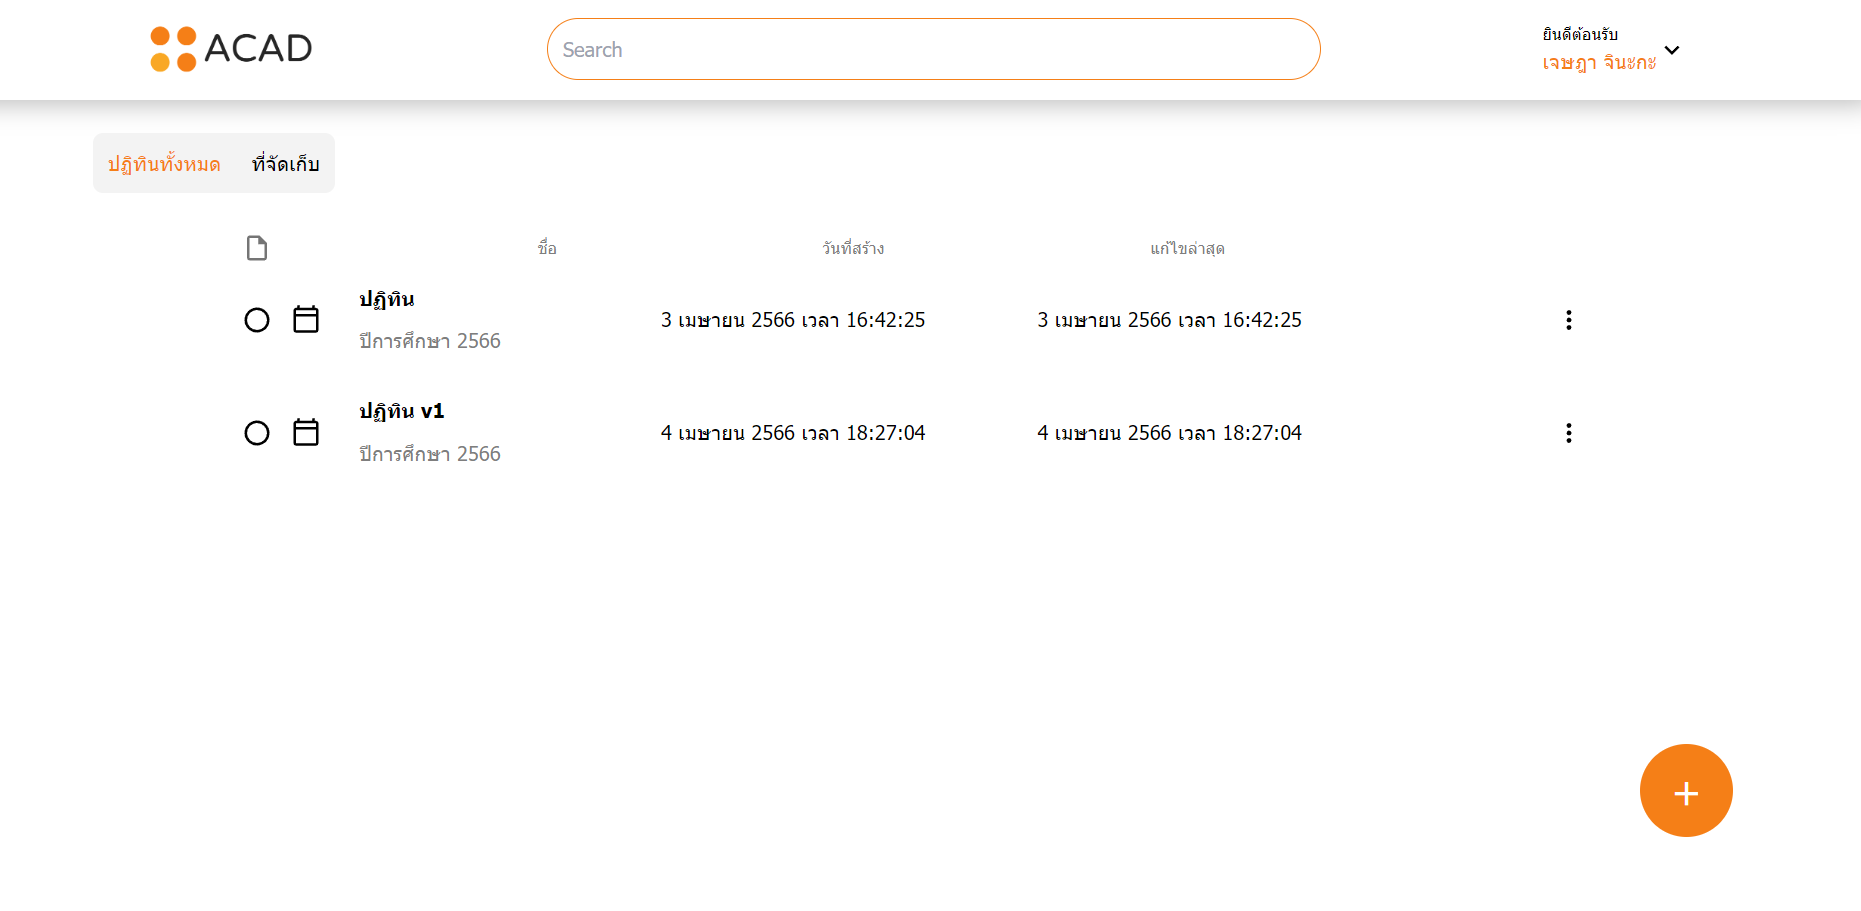
\includegraphics[width= 1\textwidth]{choose-calendar.png}
  \caption{ หน้าเลือกปฏิทิน}
  \label{fig: choose-calendar}
\end{figure}
\begin{figure}[h]
  \centering
  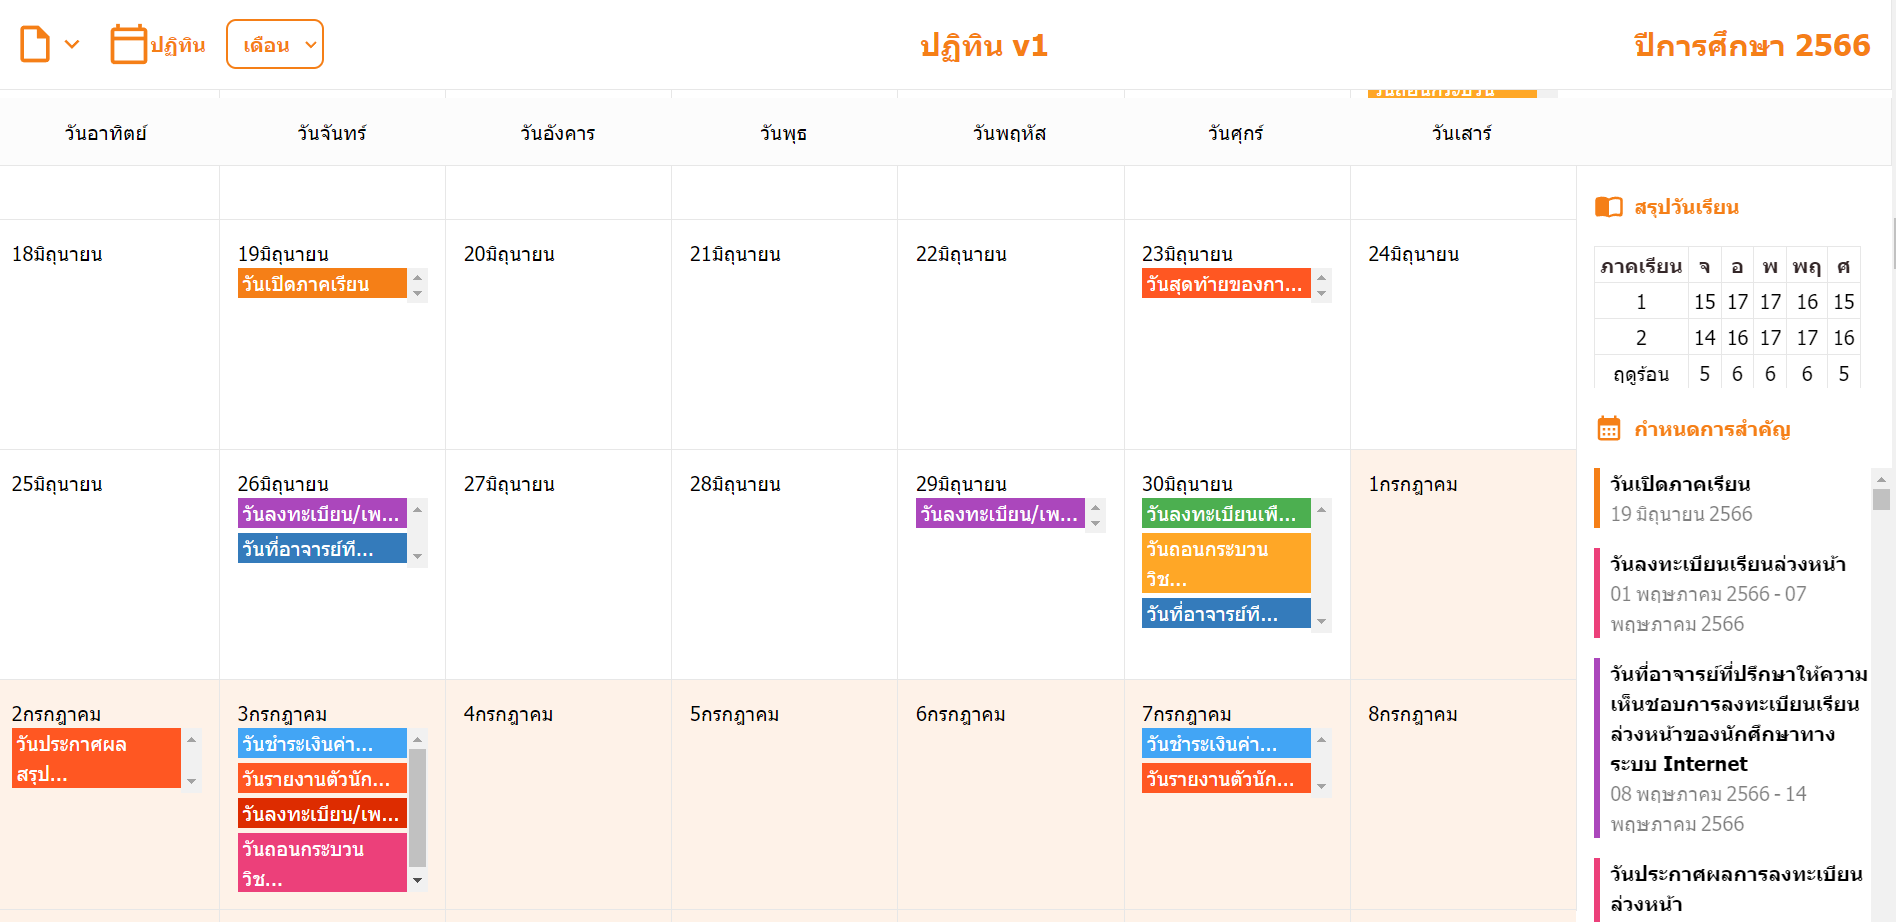
\includegraphics[width= 1\textwidth]{edit-calendar.png}
  \caption{หน้าแก้ไขร่างปฏิทิน}
  \label{fig: edit-calendar}
\end{figure}
\begin{figure}[h]
  \centering
  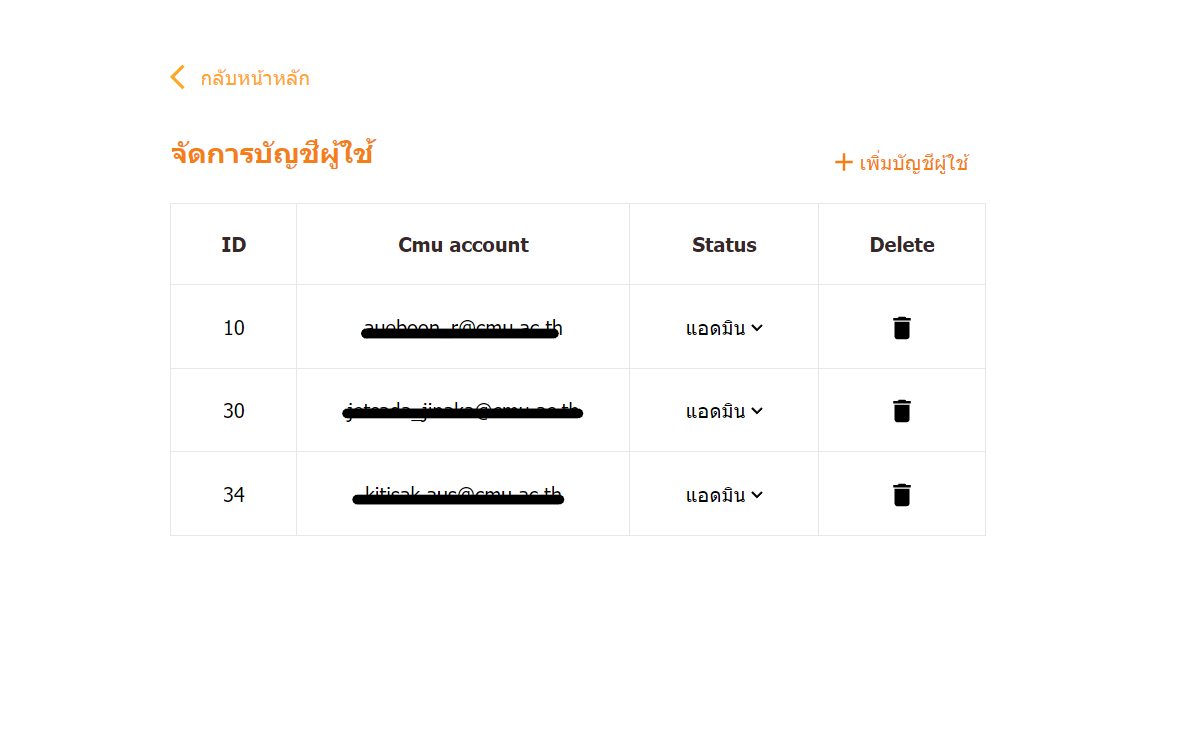
\includegraphics[width= 1\textwidth]{edit-user.png}
  \caption{หน้าจัดการผู้ใช้}
  \label{fig: edit-user}
\end{figure}
\begin{figure}[h]
  \centering
  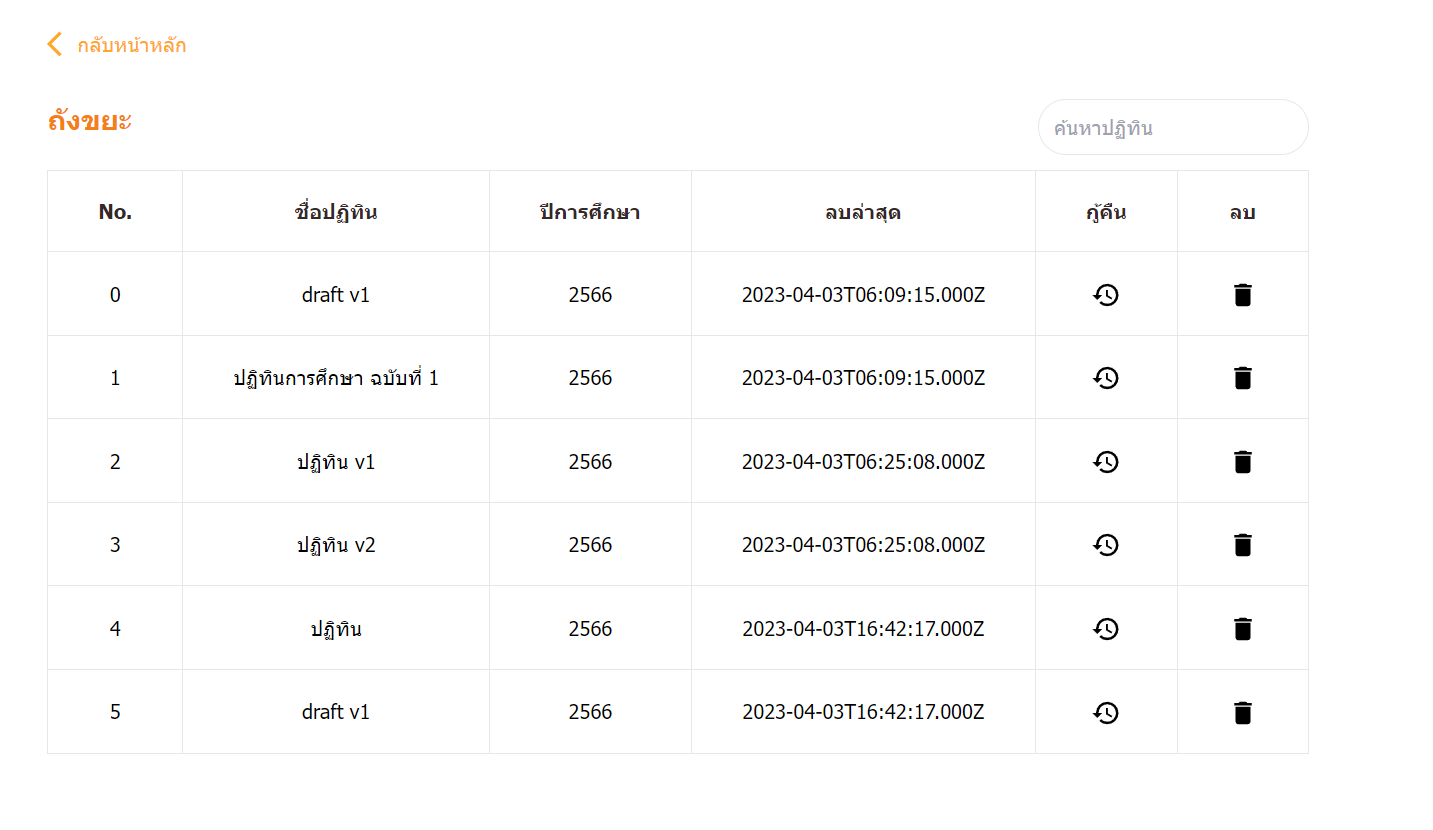
\includegraphics[width= 1\textwidth]{edit-delete.png}
  \caption{หน้าจัดการถังขยะ}
  \label{fig: edit-delete}
\end{figure}
\begin{figure}[h]
  \centering
  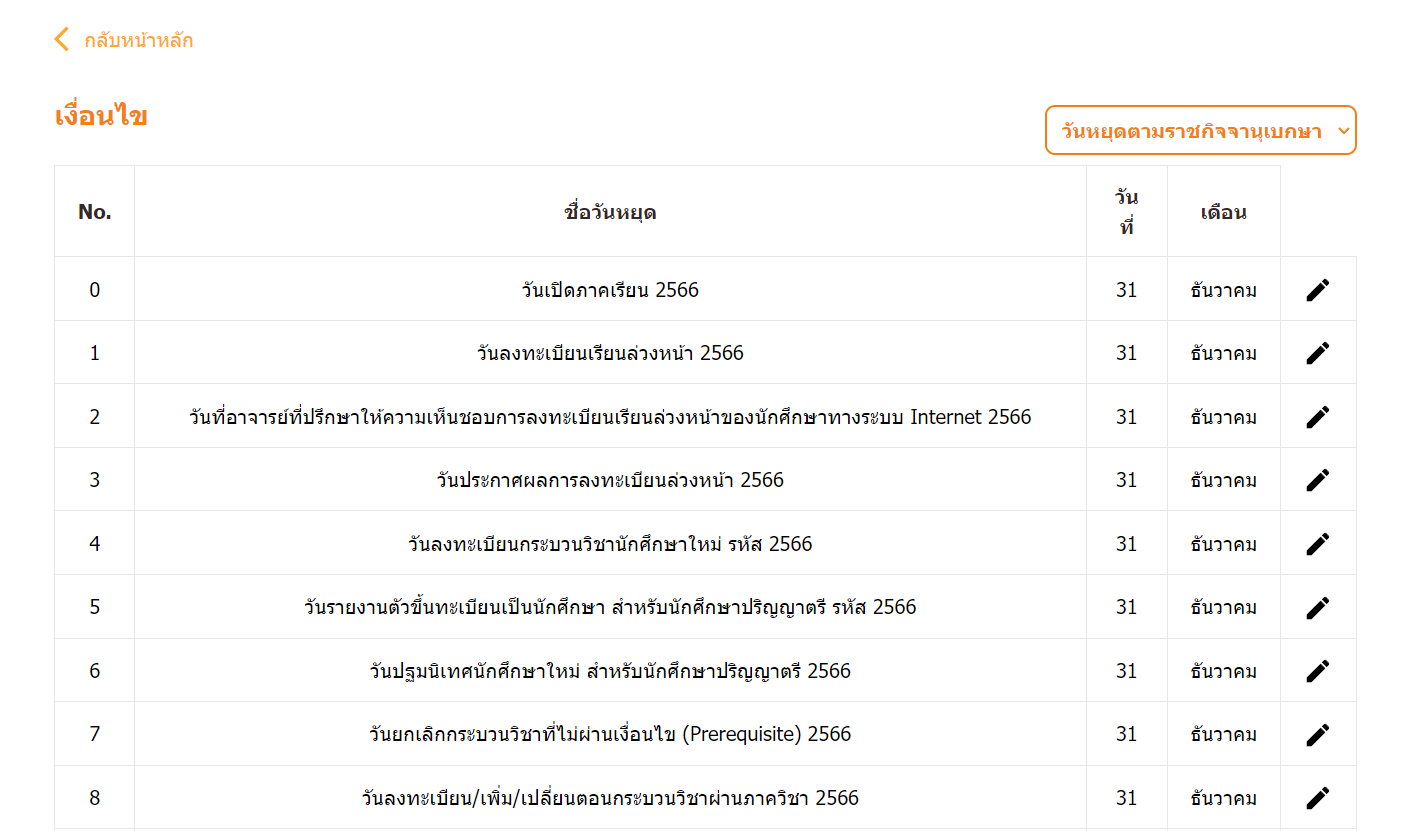
\includegraphics[width= 1\textwidth]{edit-condition.png}
  \caption{หน้าตั้งค่าเงื่อนไข}
  \label{fig: edit-condition}
\end{figure}
\clearpage

\newpage
\paragraph{การเข้าสู่ระบบ}
การใช้งานของระบบนั้น ระบบจะจำกัดผู้ที่เข้าได้เฉพาะผู้ที่มีสิทธิ์ในการแก้ไขจัดการร่างปฏิทินนี้ และ จะต้องเป็นบุคลลากรที่มีcmuitaccount เท่านั้น เพื่อเป็นการยืนยันการเข้าสู่ระบบ
เมื่อเข้าสู่ระบบเรียบบร้อยแล้วนั้น ผู้เข้าใช้งานจะเห็นหน้า เลือกปฏิทินการศึกษา (รูปที่ 3.2) โดยผู้ใช้สามารถทำการสร้าง ร่างปฏิทิน ใหม่ เพื่อแก้ไข หรือ 
สามารถเข้าสู่การแก้ไขปฏิทินที่มีเดิมอยู่แล้ว
\ref*{fig: login-page}
\begin{figure}[h]
  \centering
  
\includegraphics[width= 1\textwidth]{cmu-oauth.png}
  \caption{หน้าเข้าสู่ระบบของ CMU OAuth}
  \label{fig: oauth-login}
\end{figure}

\begin{figure}[h]
  \centering
  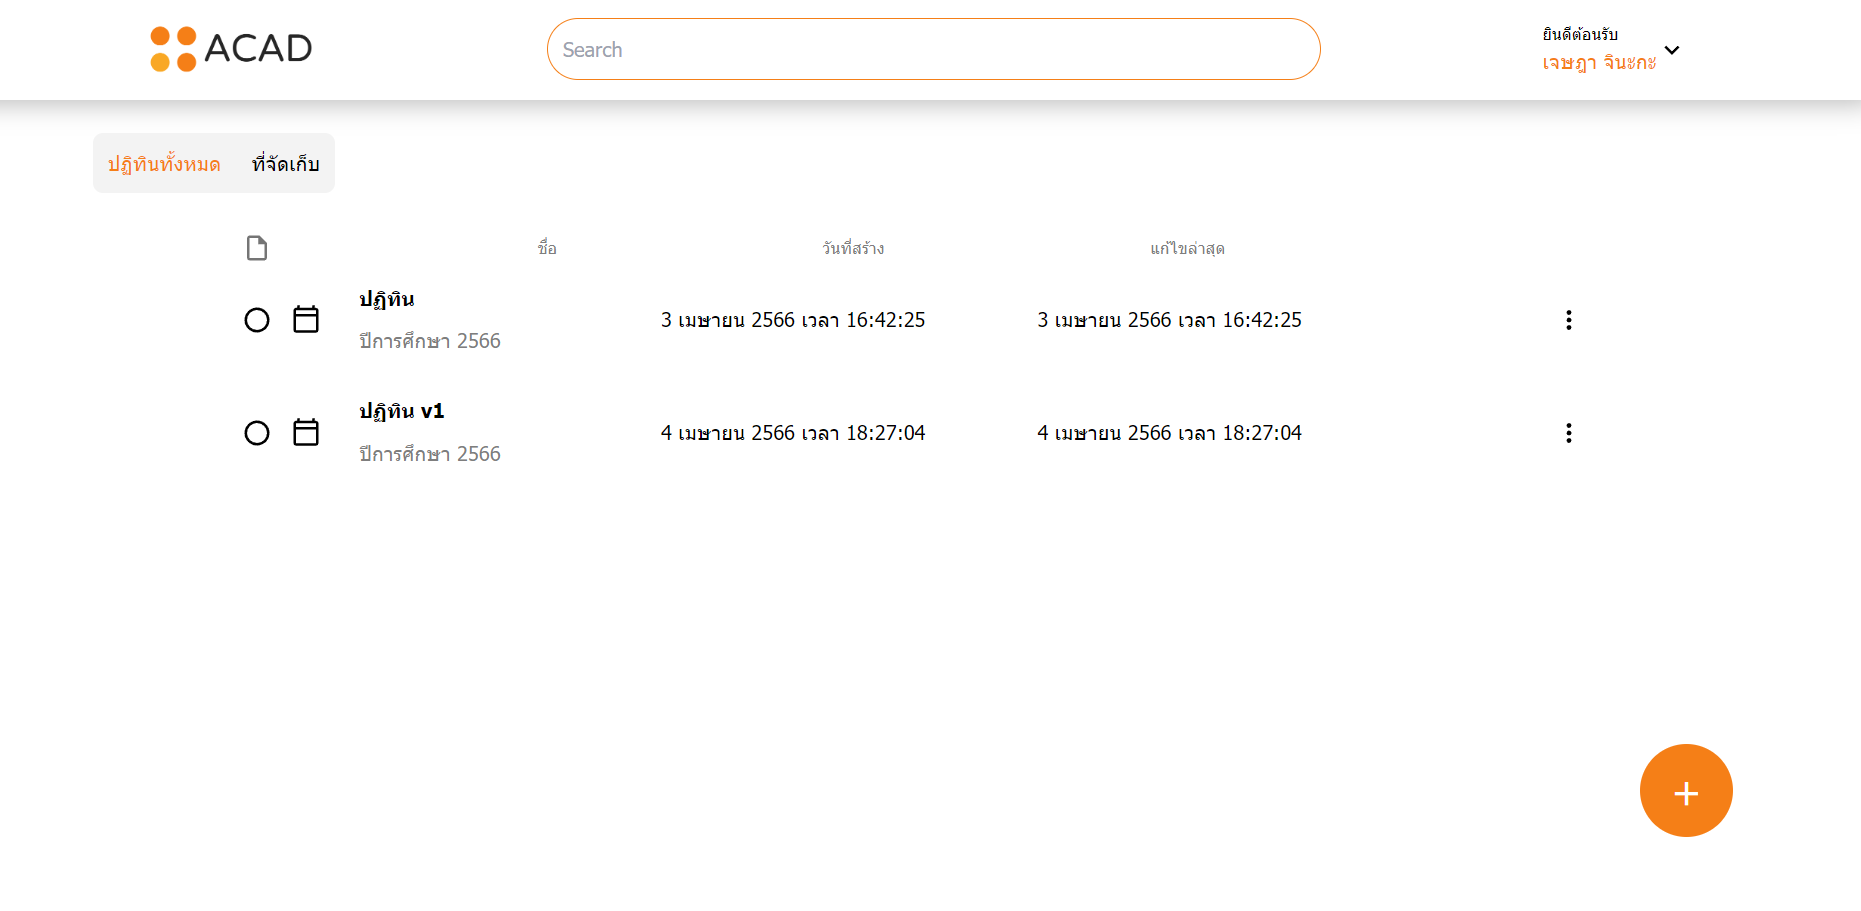
\includegraphics[width= 1\textwidth]{choose-calendar.png}
  \caption{หน้าเลือกปฏิทิน}
  \label{fig: choose-calendar-page}
\end{figure}

\section*{ตรวจสอบเงื่อนไข}

\section*{การออกแบบโครงสร้างพื้นฐานของข้อมูล}

\section*{ขั้นตอนการดําเนินงาน}





